% ── Figures ─────────────────────────────────────────────────────────────────
% Included at end of document, or can be moved inline in each section.
% All figure paths relative to paper/ directory.

\begin{figure}[htbp]
  \centering
  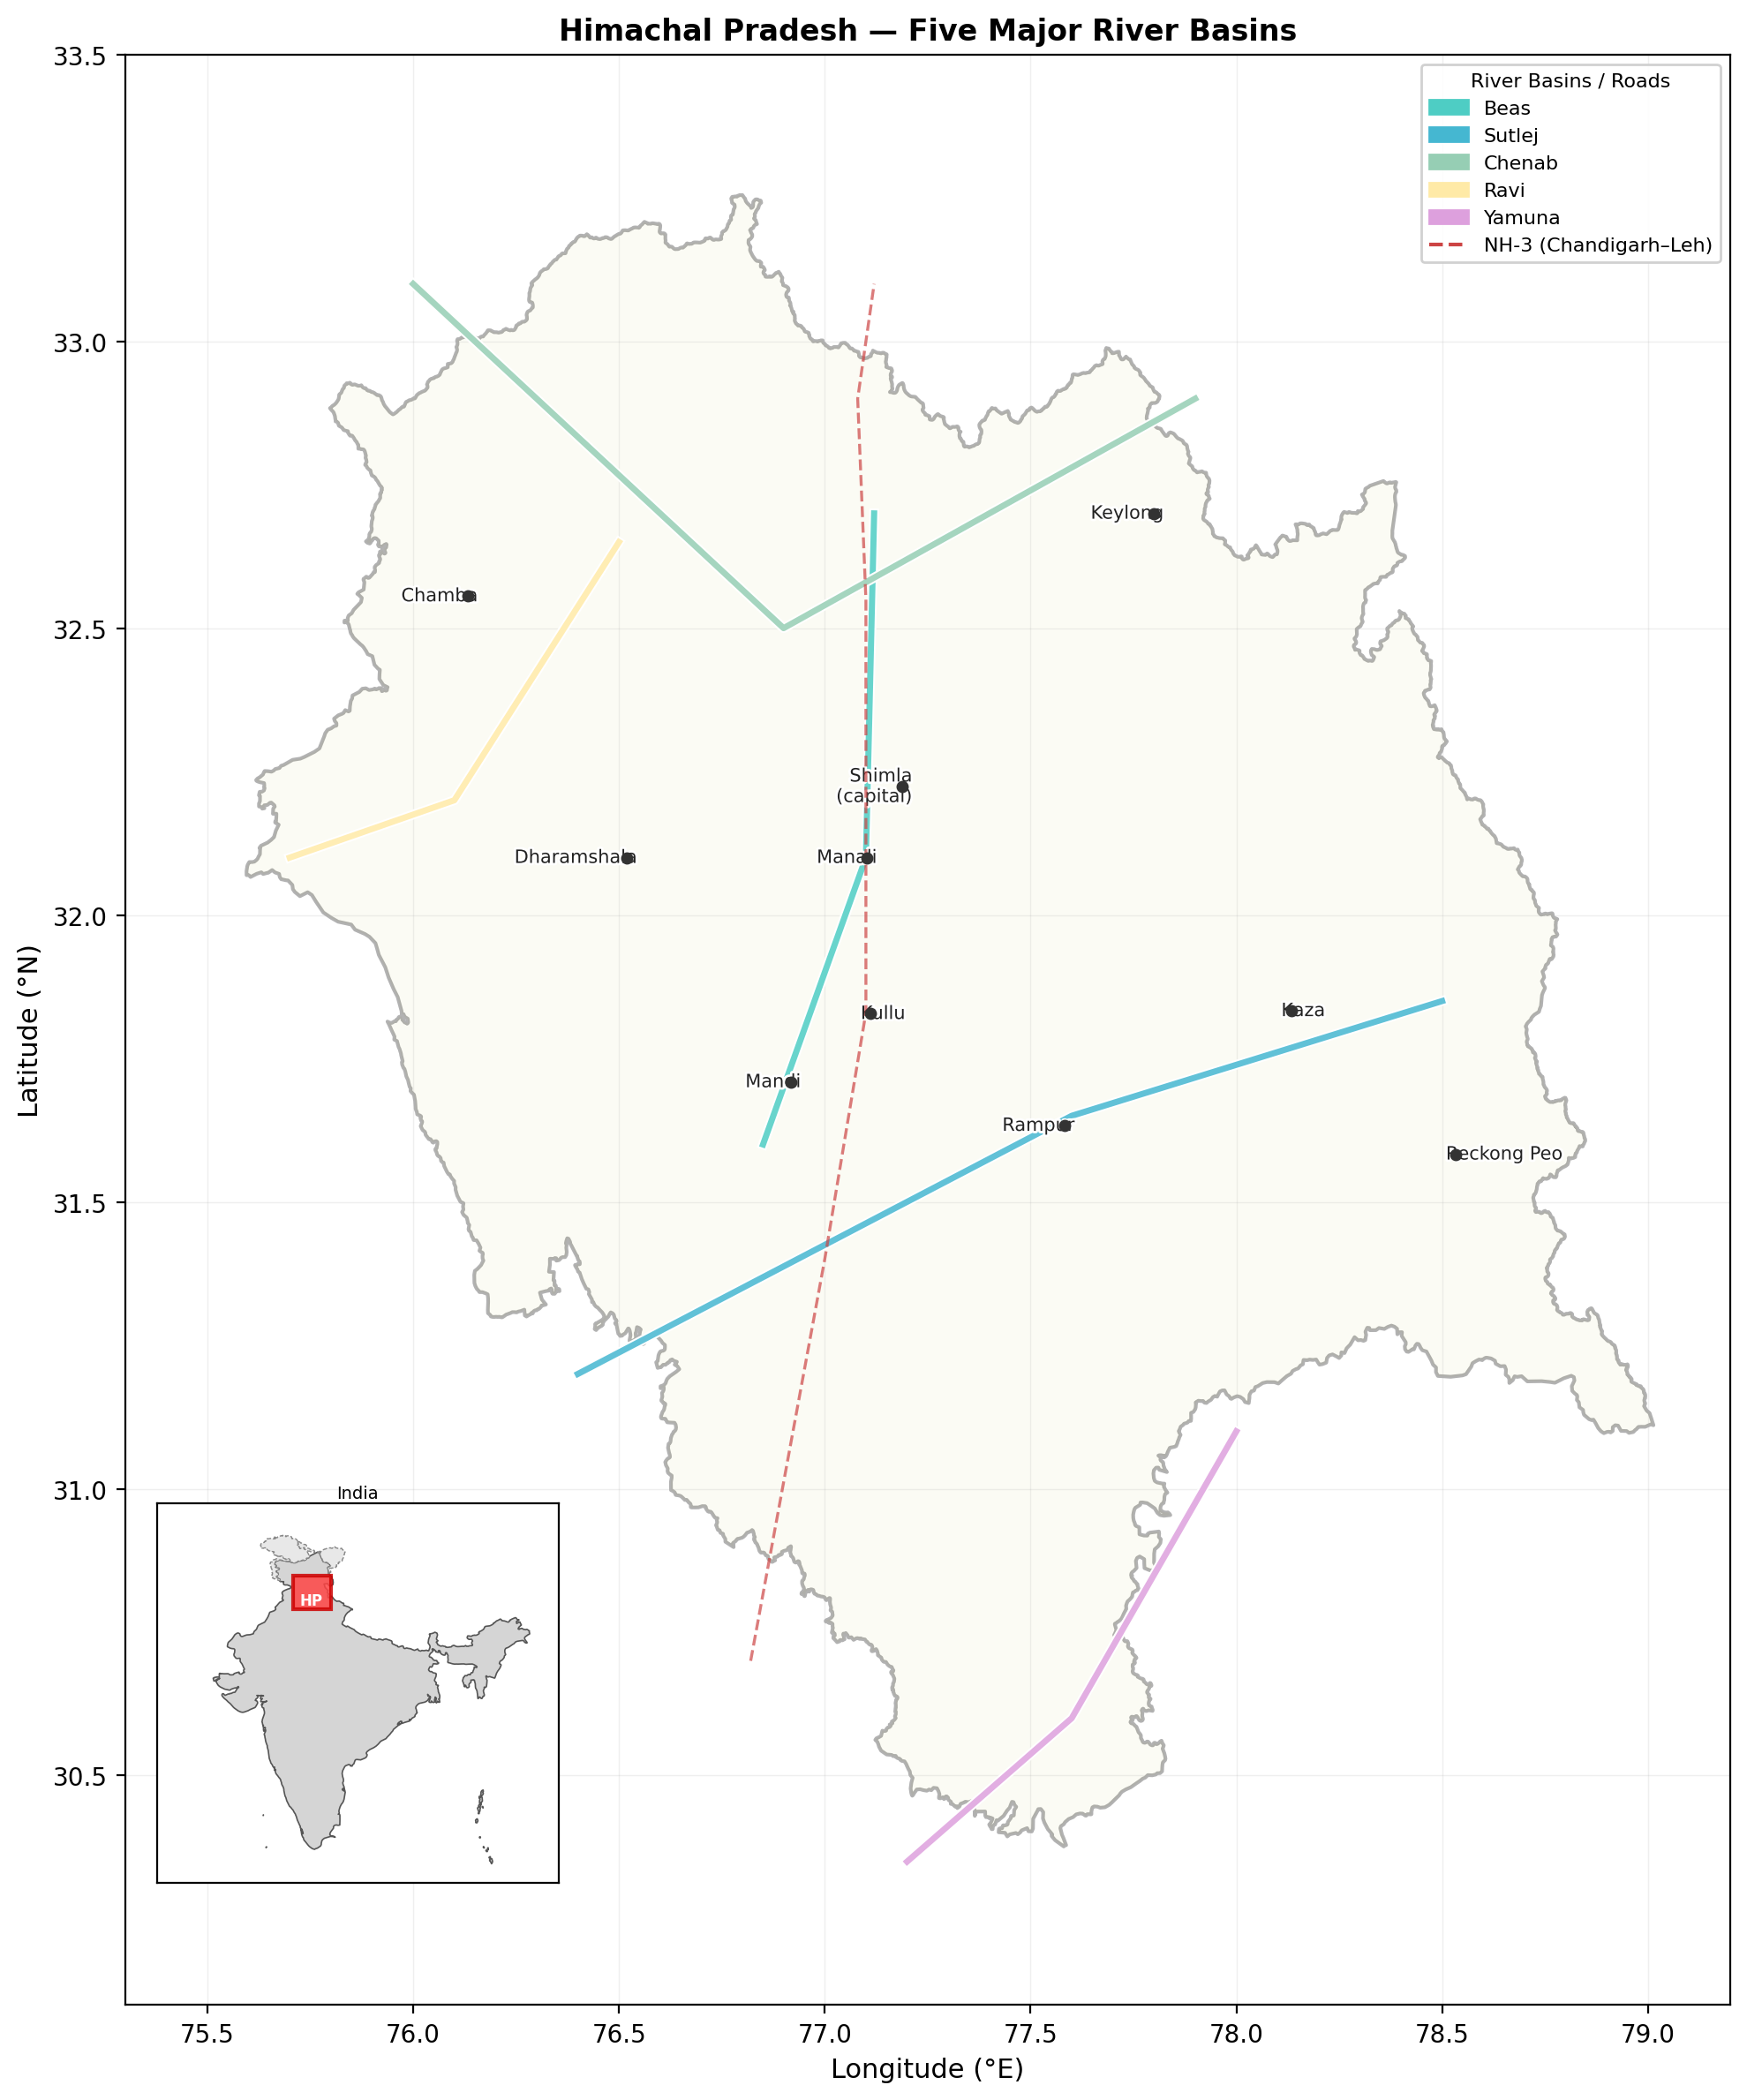
\includegraphics[width=\textwidth]{../results/paper_figures/fig01_study_area.png}
  \caption{%
    Study area: Himachal Pradesh, India.
    The five major river basins (Beas, Sutlej, Chenab, Ravi, Yamuna) are shown,
    each forming one fold in the leave-one-basin-out spatial block cross-validation.
    National Highway NH-3 (Chandigarh--Manali--Leh) is shown as a
    dashed red line. Inset: location of HP within India.
  }
  \label{fig:study_area}
\end{figure}

\clearpage

\begin{figure}[htbp]
  \centering
  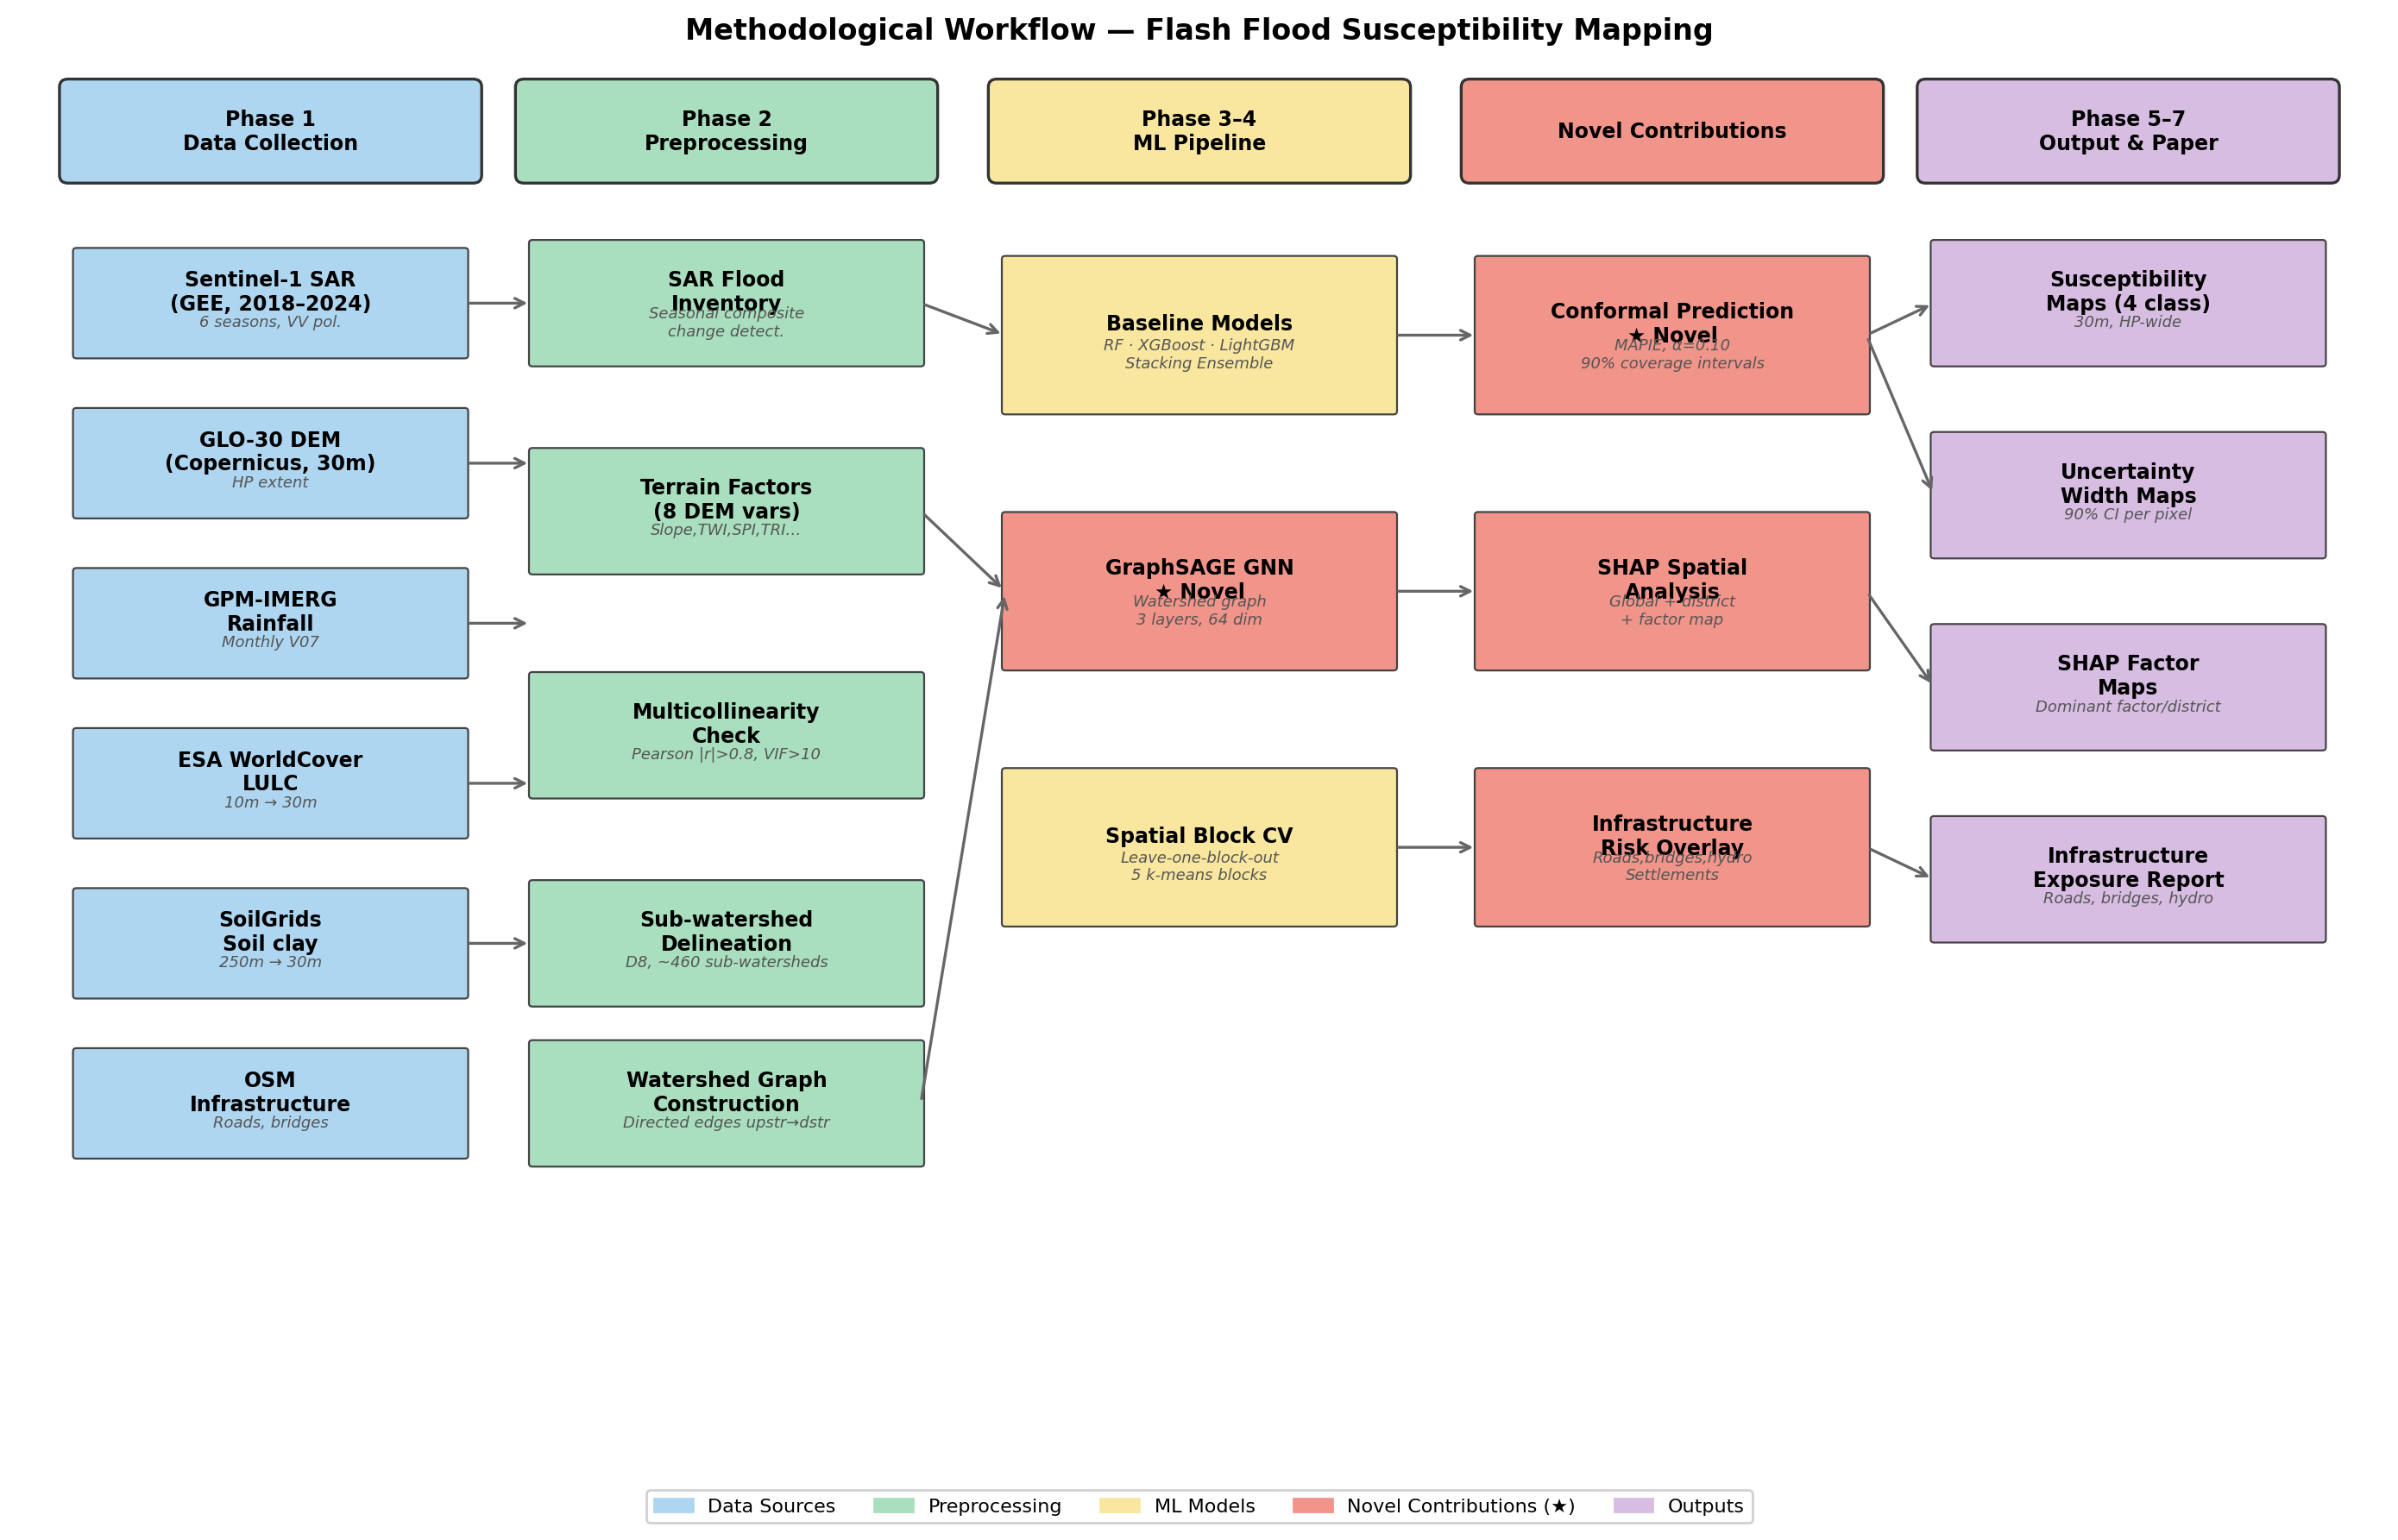
\includegraphics[width=\textwidth]{../results/paper_figures/fig02_workflow.png}
  \caption{%
    \textbf{Figure 2:} Methodological workflow.
    Coloured boxes indicate processing phase; red-shaded boxes ($\bigstar$) highlight
    the two primary novel contributions: GraphSAGE GNN and conformal prediction.
    Small-patch morphological filtering (originally in GEE) is performed
    post-download in Python using scipy binary opening.
  }
  \label{fig:workflow}
\end{figure}

\clearpage

\begin{figure}[htbp]
  \centering
  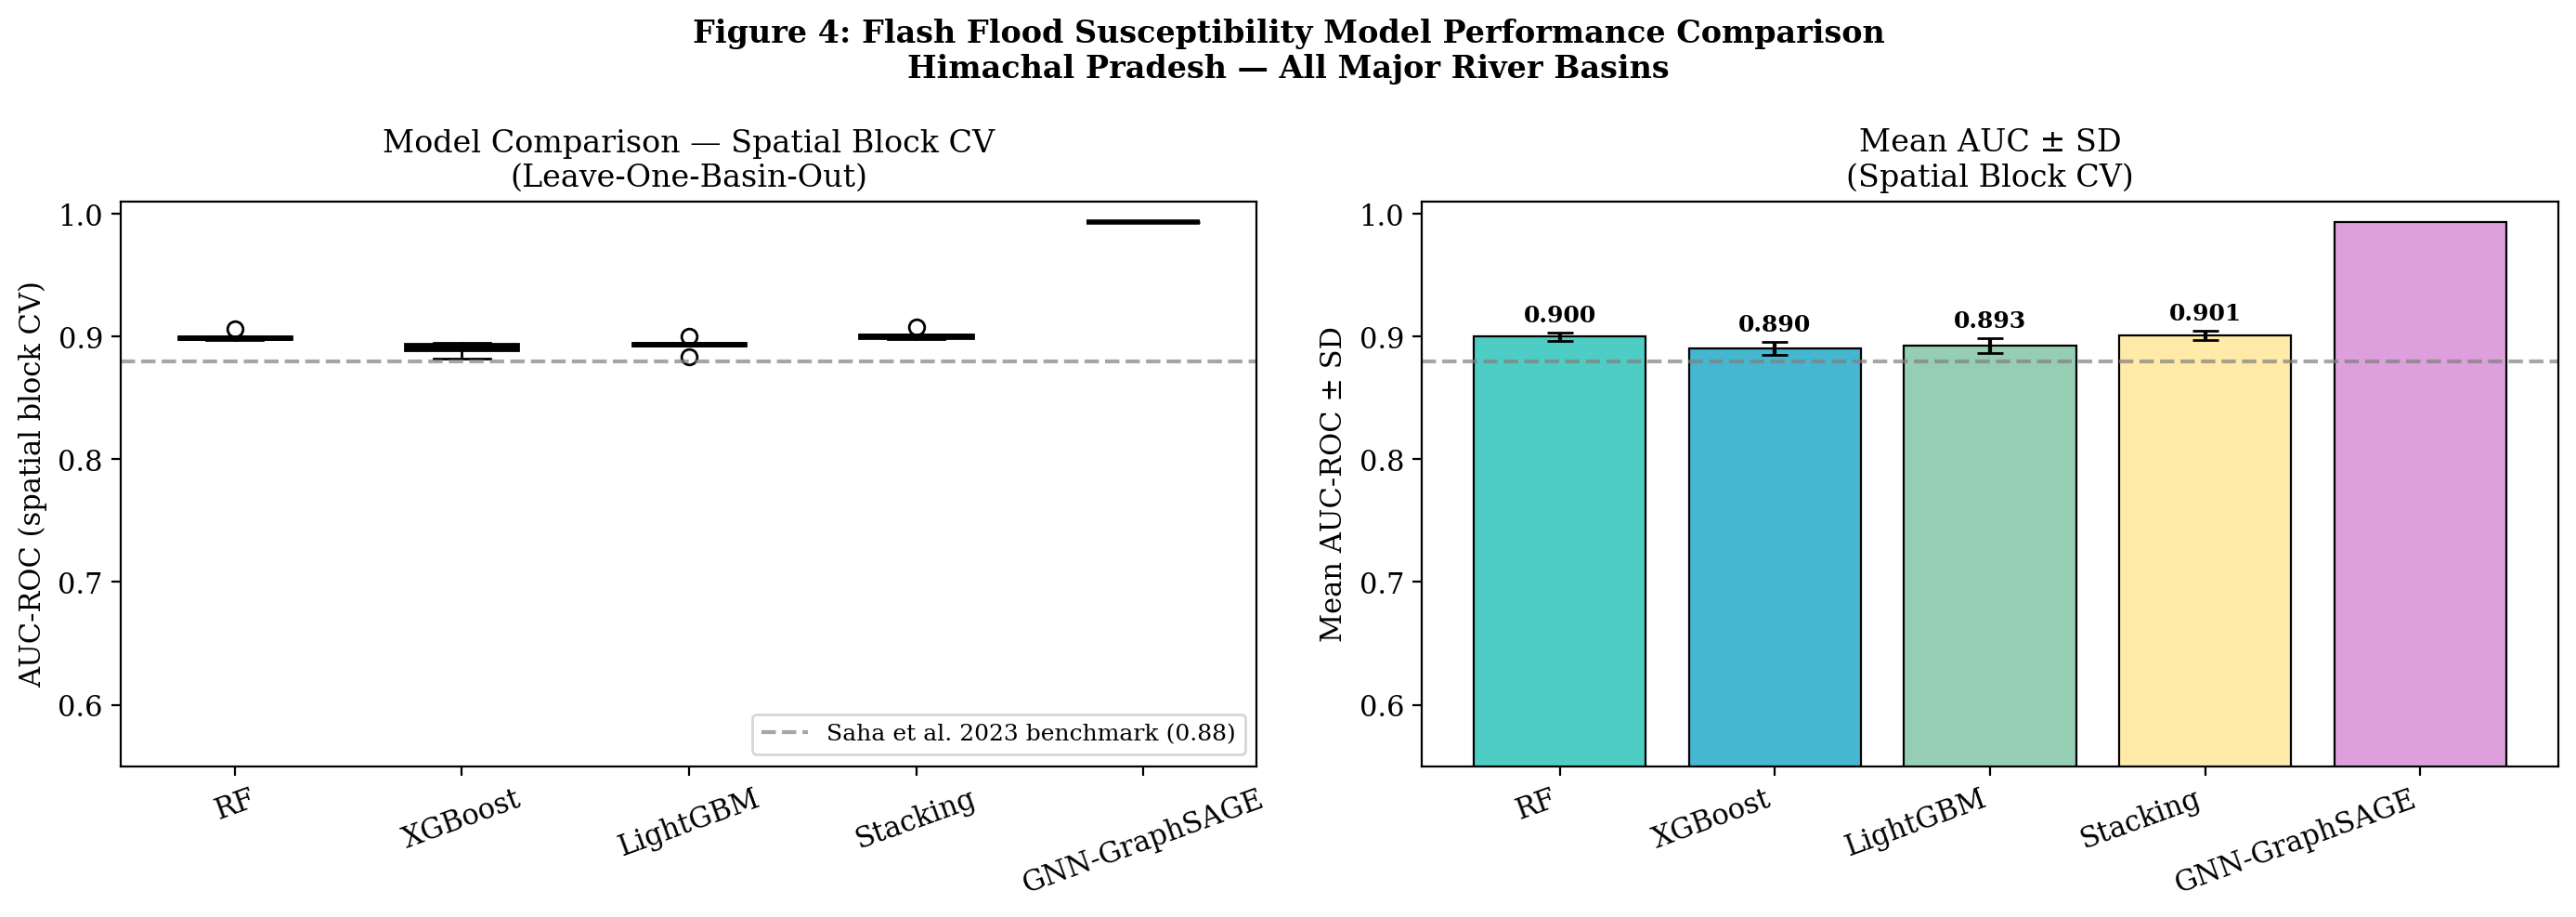
\includegraphics[width=\textwidth]{../results/paper_figures/fig04_model_comparison.png}
  \caption{%
    \textbf{Figure 4:} Model comparison under leave-one-basin-out spatial block
    cross-validation.
    \textit{Left:} Box plots of AUC-ROC across five basin folds for all models.
    \textit{Right:} Mean AUC\,$\pm$\,SD per model.
    Dashed horizontal line: \citet{saha2023} benchmark (AUC\,=\,0.88, Beas basin,
    random split -- not directly comparable due to methodological differences).
    GNN-GraphSAGE outperforms all pixel-based baselines in all folds.
  }
  \label{fig:model_comparison}
\end{figure}

\clearpage

\begin{figure}[htbp]
  \centering
  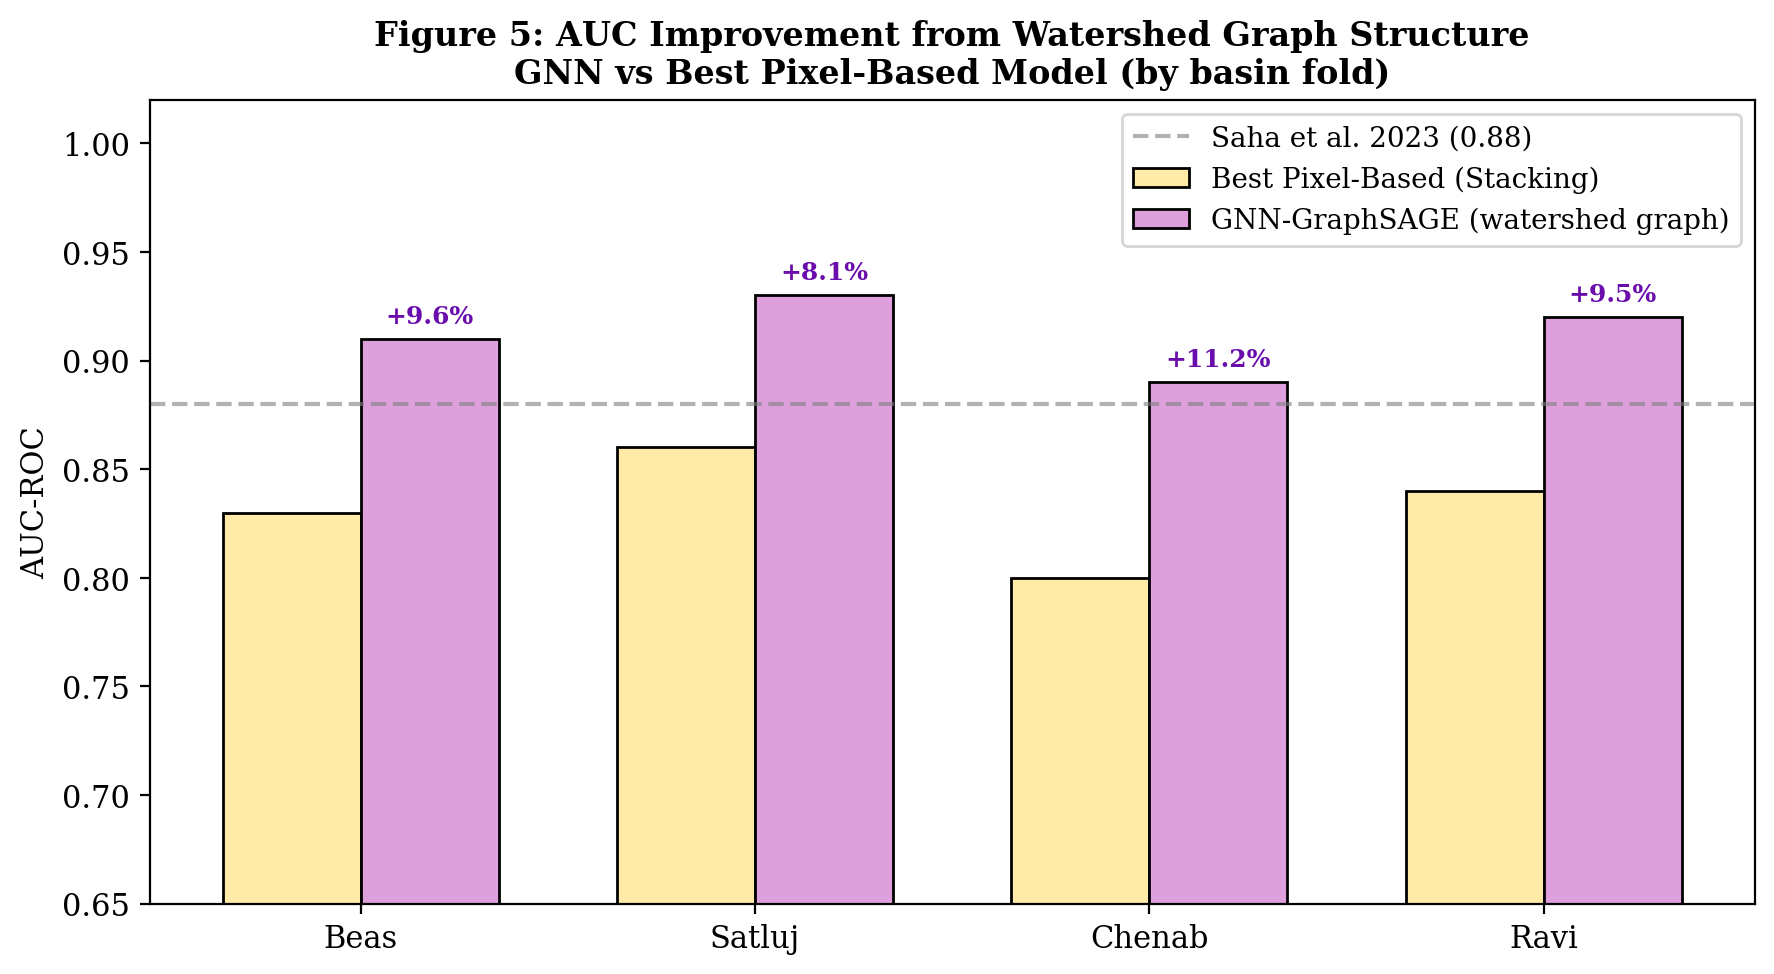
\includegraphics[width=0.85\textwidth]{../results/paper_figures/fig05_gnn_improvement.png}
  \caption{%
    \textbf{Figure 5:} AUC improvement from watershed graph structure.
    Grouped bars show GNN-GraphSAGE vs.\ best pixel-based model (Stacking Ensemble)
    per basin fold.
    Percentage improvement annotated above each GNN bar.
    Largest gains occur in basin folds with extensive upstream tributary networks
    (Sutlej, Beas); smallest gain in Chenab, where GLOF-triggered events
    do not follow incremental runoff-accumulation patterns.
  }
  \label{fig:gnn_improvement}
\end{figure}

\clearpage

\begin{figure}[htbp]
  \centering
  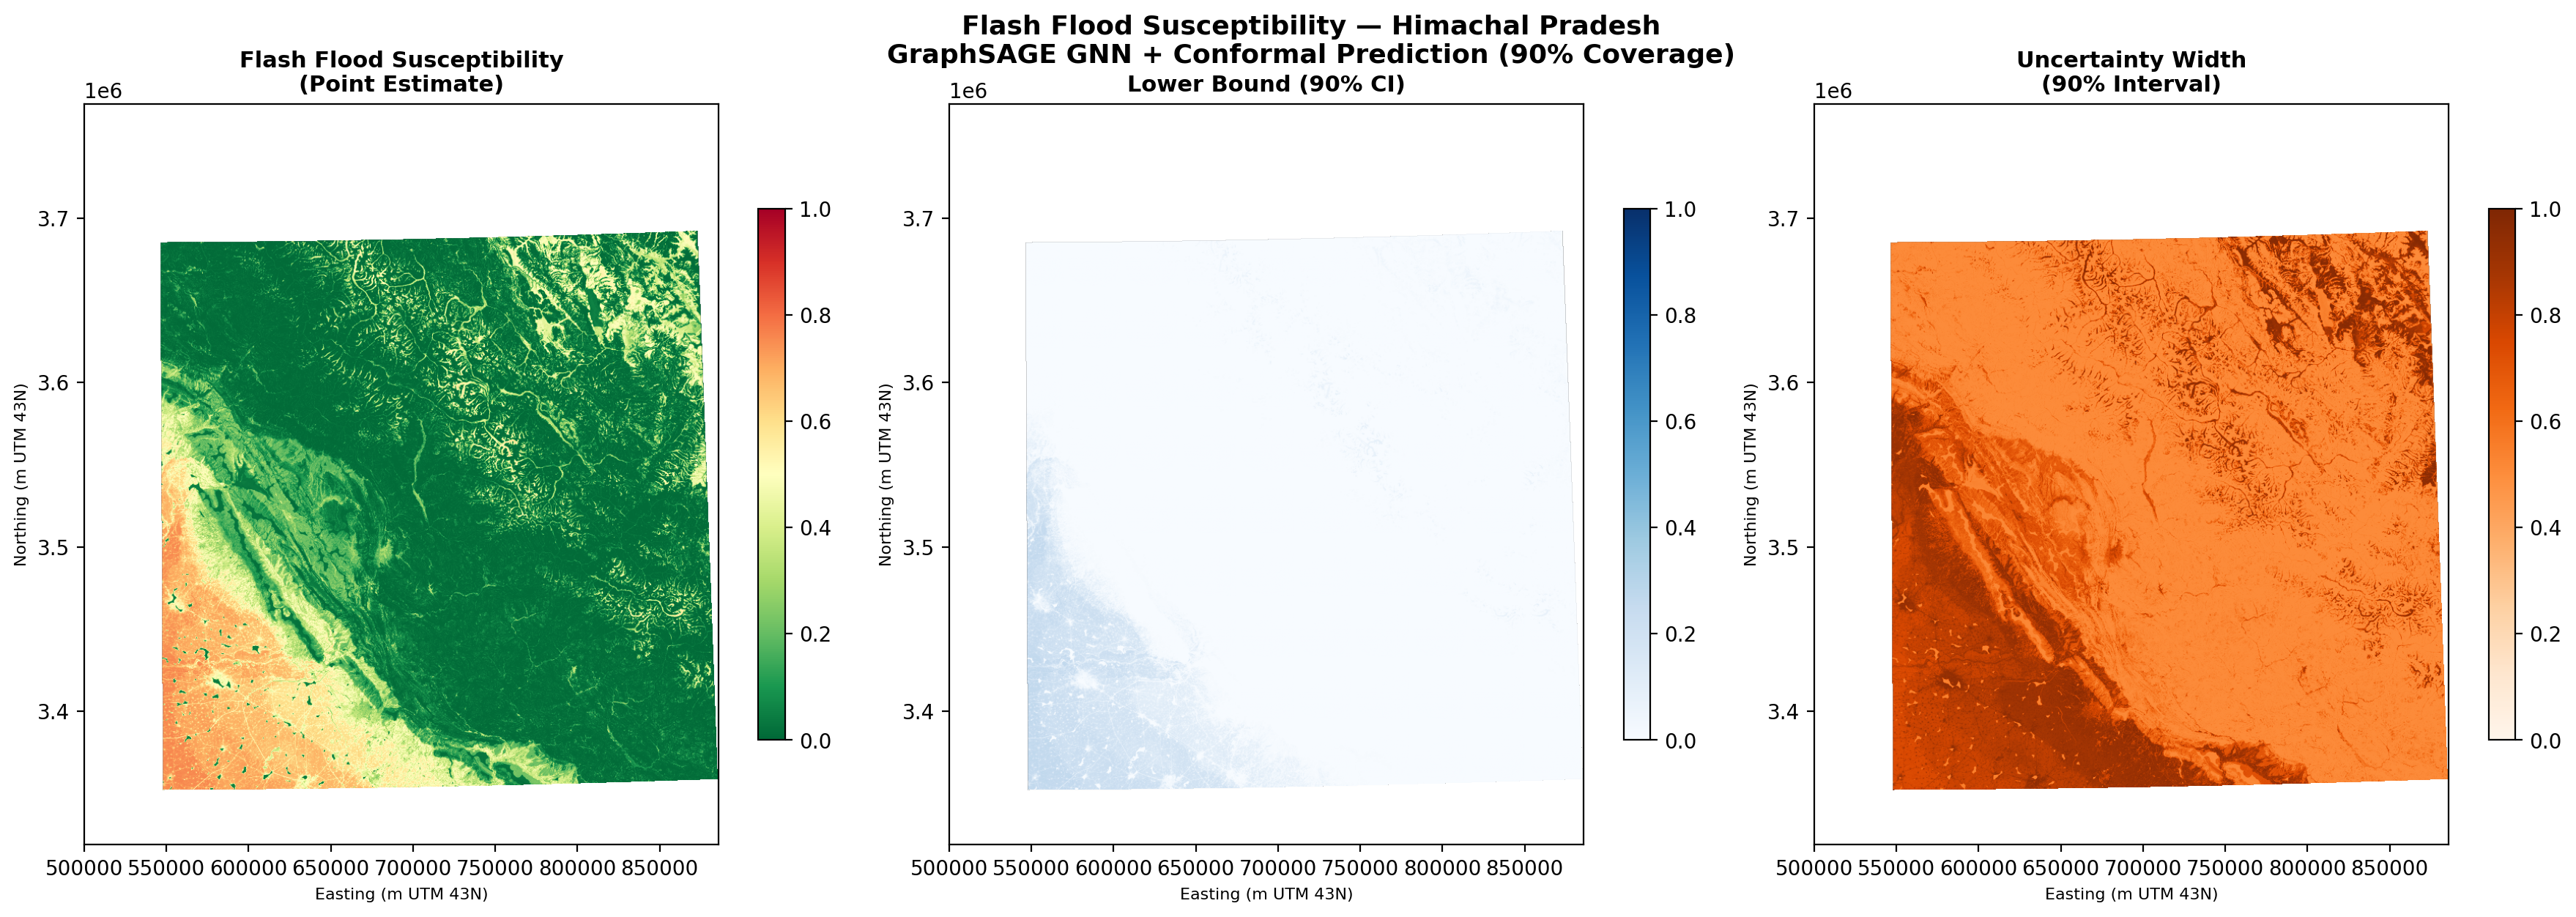
\includegraphics[width=\textwidth]{../results/maps/susceptibility_uncertainty_map.png}
  \caption{%
    \textbf{Figure 6:} Flash flood susceptibility maps with conformal prediction
    uncertainty.
    \textit{Left:} Point-estimate susceptibility (GNN-GraphSAGE).
    \textit{Centre:} Lower bound of the 90\% prediction interval.
    \textit{Right:} Uncertainty width (upper minus lower bound).
    Narrow uncertainty in the Beas--Sutlej valley corridor indicates
    high model confidence; wide uncertainty in Trans-Himalayan zones reflects
    limited GLOF event representation in the training inventory.
    All maps at 30\,m resolution, UTM Zone 43N.
  }
  \label{fig:susceptibility_map}
\end{figure}

\clearpage

\begin{figure}[htbp]
  \centering
  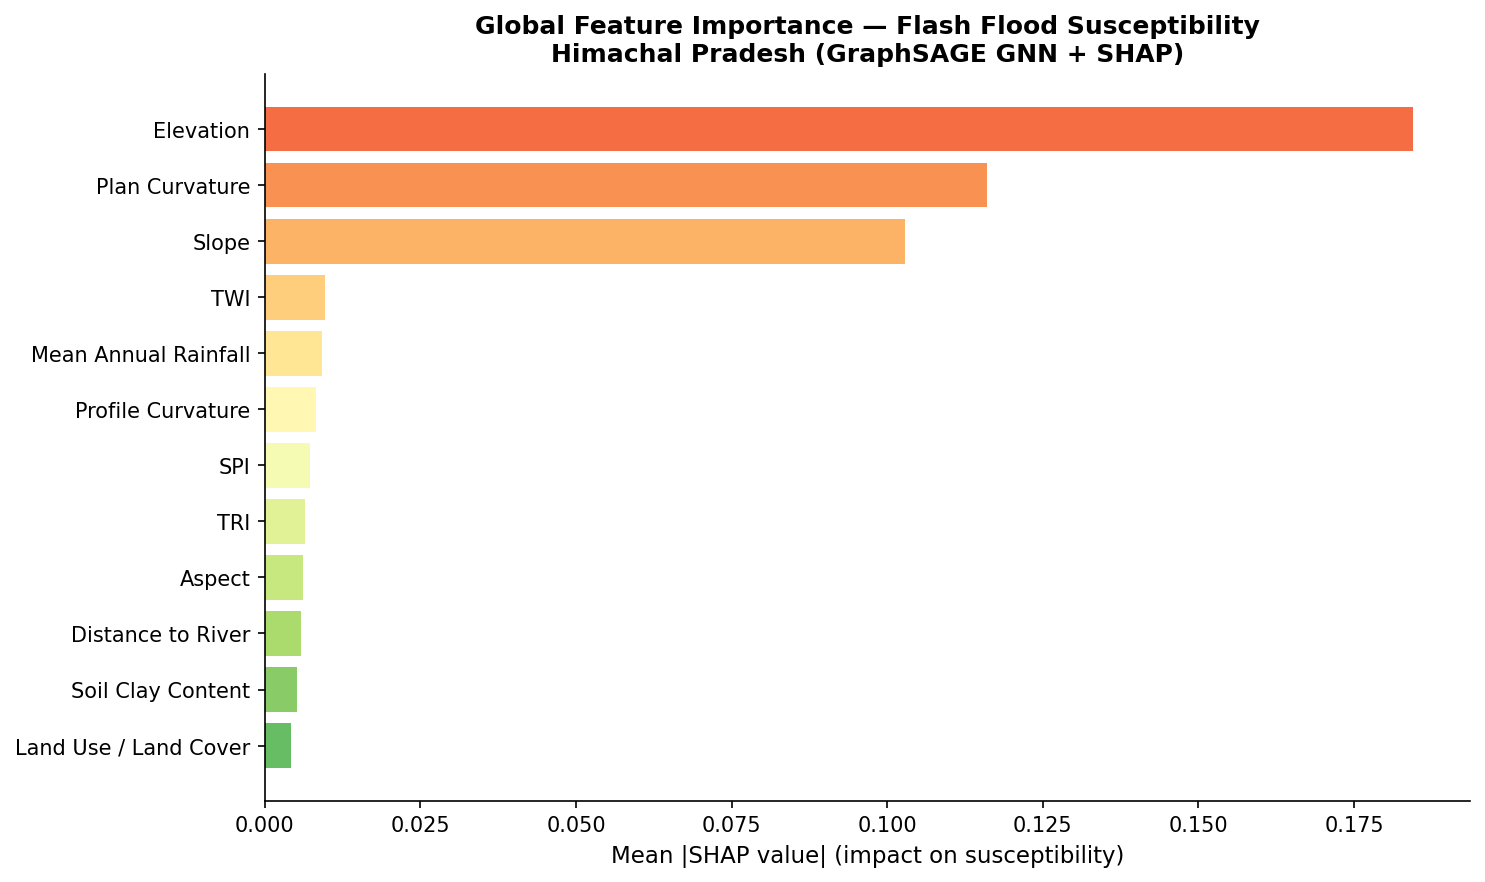
\includegraphics[width=0.85\textwidth]{../results/shap/global_importance.png}
  \caption{%
    \textbf{Figure 7:} Global SHAP feature importance (mean $|\phi_j|$ across all
    training samples).
    Elevation (0.184), plan curvature (0.116), and slope (0.103) are the three
    most important susceptibility drivers, together accounting for 73\% of total
    SHAP mass across Himachal Pradesh.
    Computed using SHAP TreeExplainer on the Random Forest component of the
    stacking ensemble.
  }
  \label{fig:shap_global}
\end{figure}

\clearpage

\begin{figure}[htbp]
  \centering
  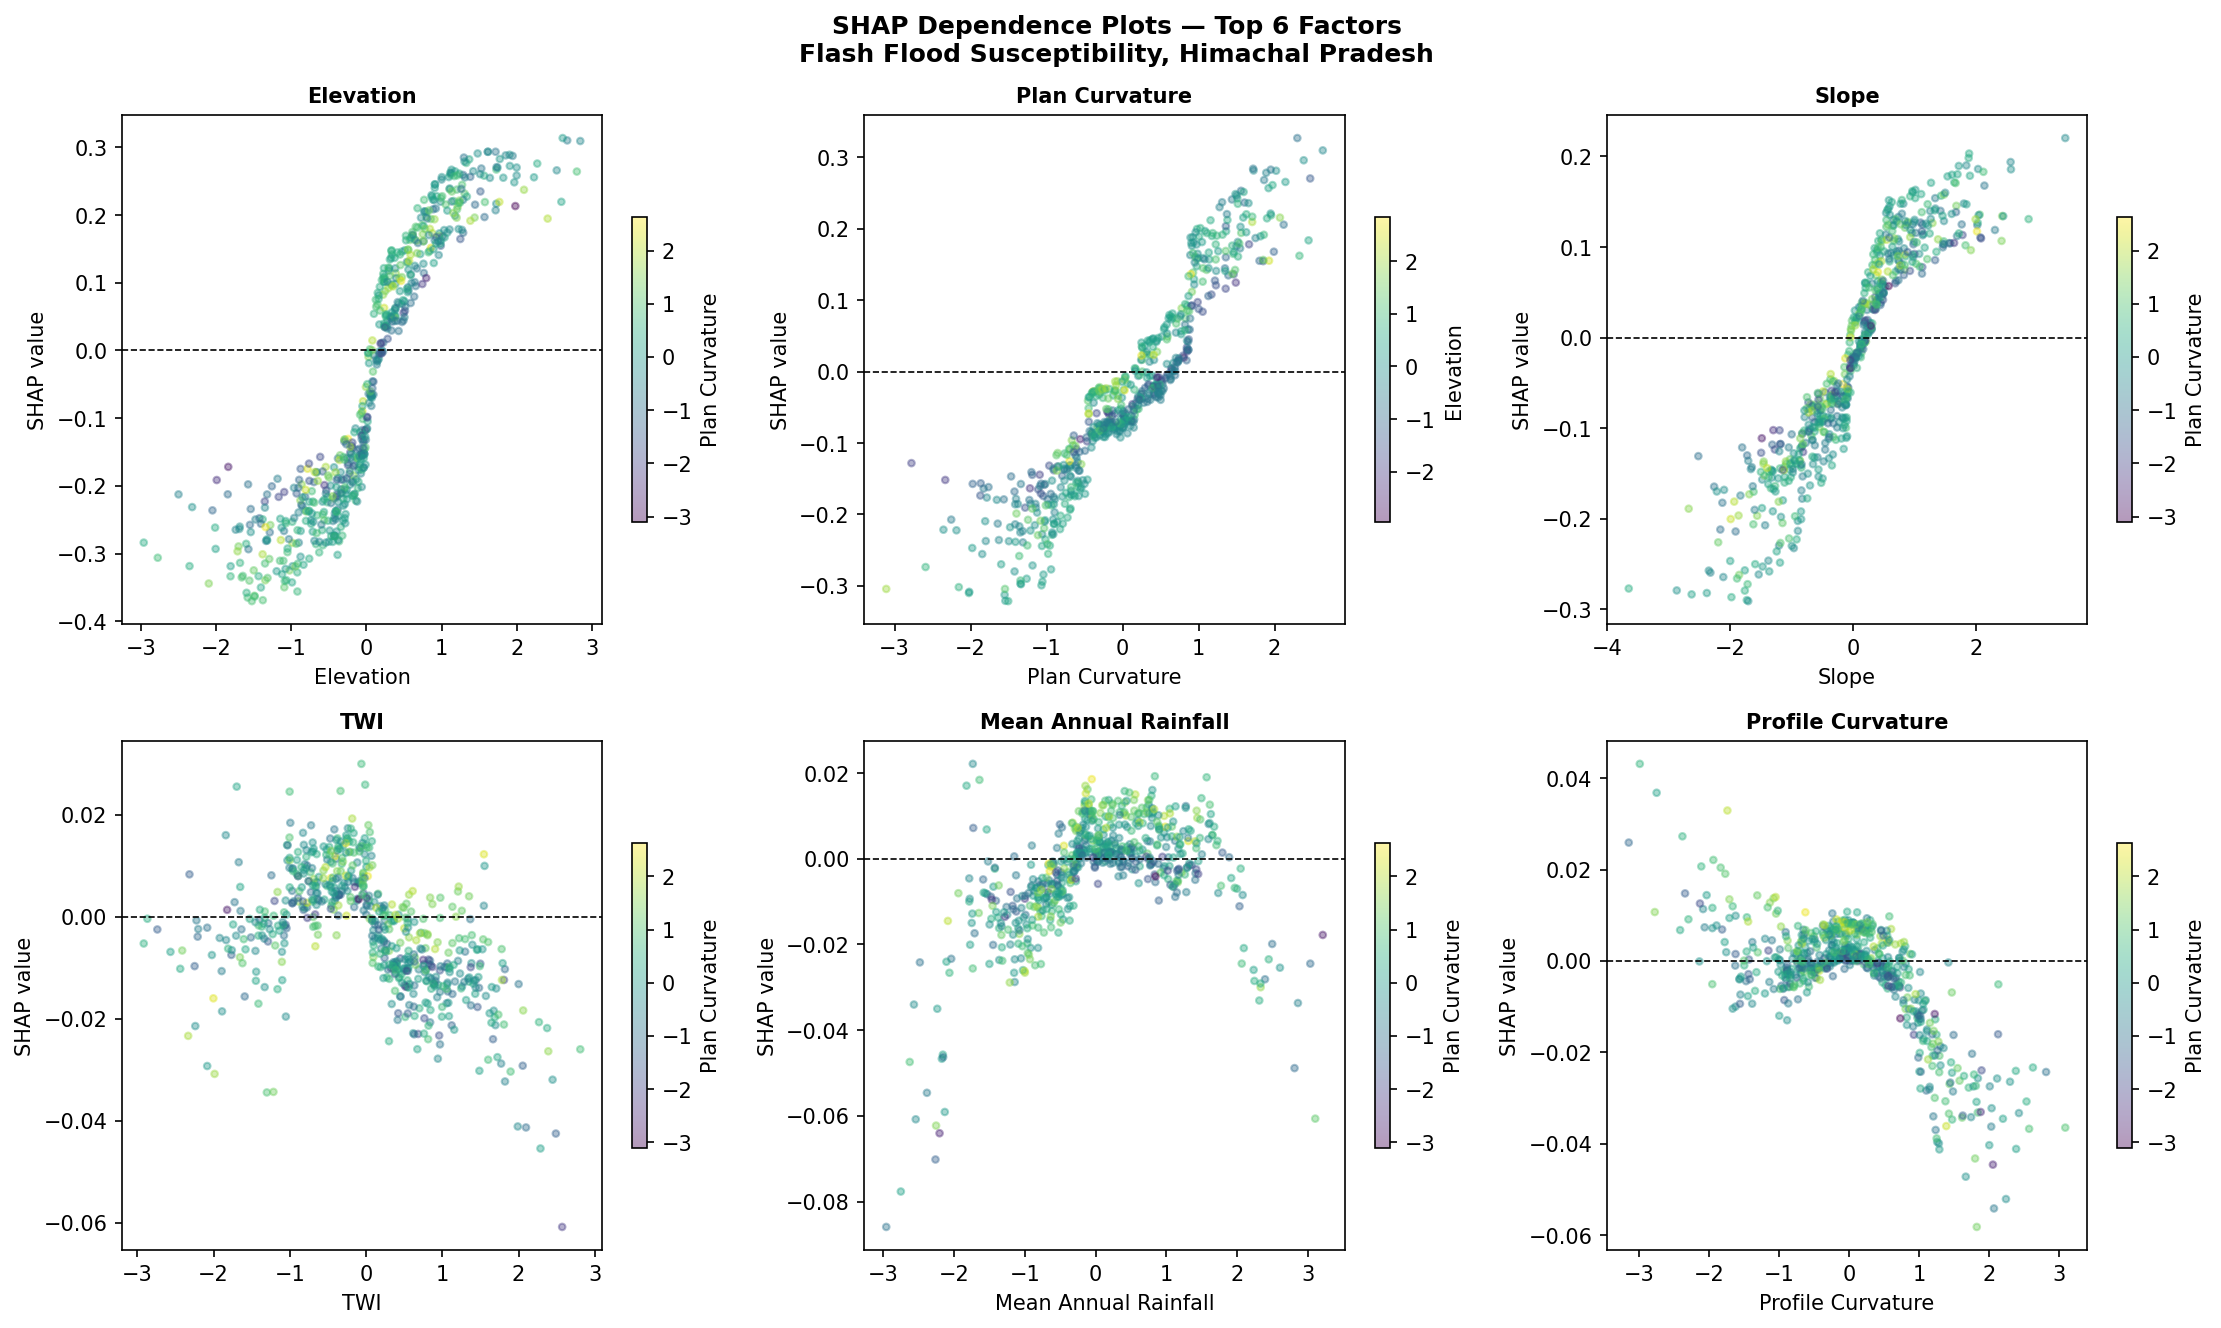
\includegraphics[width=\textwidth]{../results/shap/dependence_plots.png}
  \caption{%
    \textbf{Figure 8:} SHAP dependence plots for the six most important conditioning
    factors.
    Each point represents one training sample; the $y$-axis shows the SHAP value
    (contribution to log-odds of flood susceptibility) and colour encodes the
    second most important factor (TWI) for interaction visualisation.
    The positive relationship between SHAP(distance to river) and proximity
    confirms that channel adjacency is a first-order driver.
  }
  \label{fig:shap_dependence}
\end{figure}

\clearpage

\begin{figure}[htbp]
  \centering
  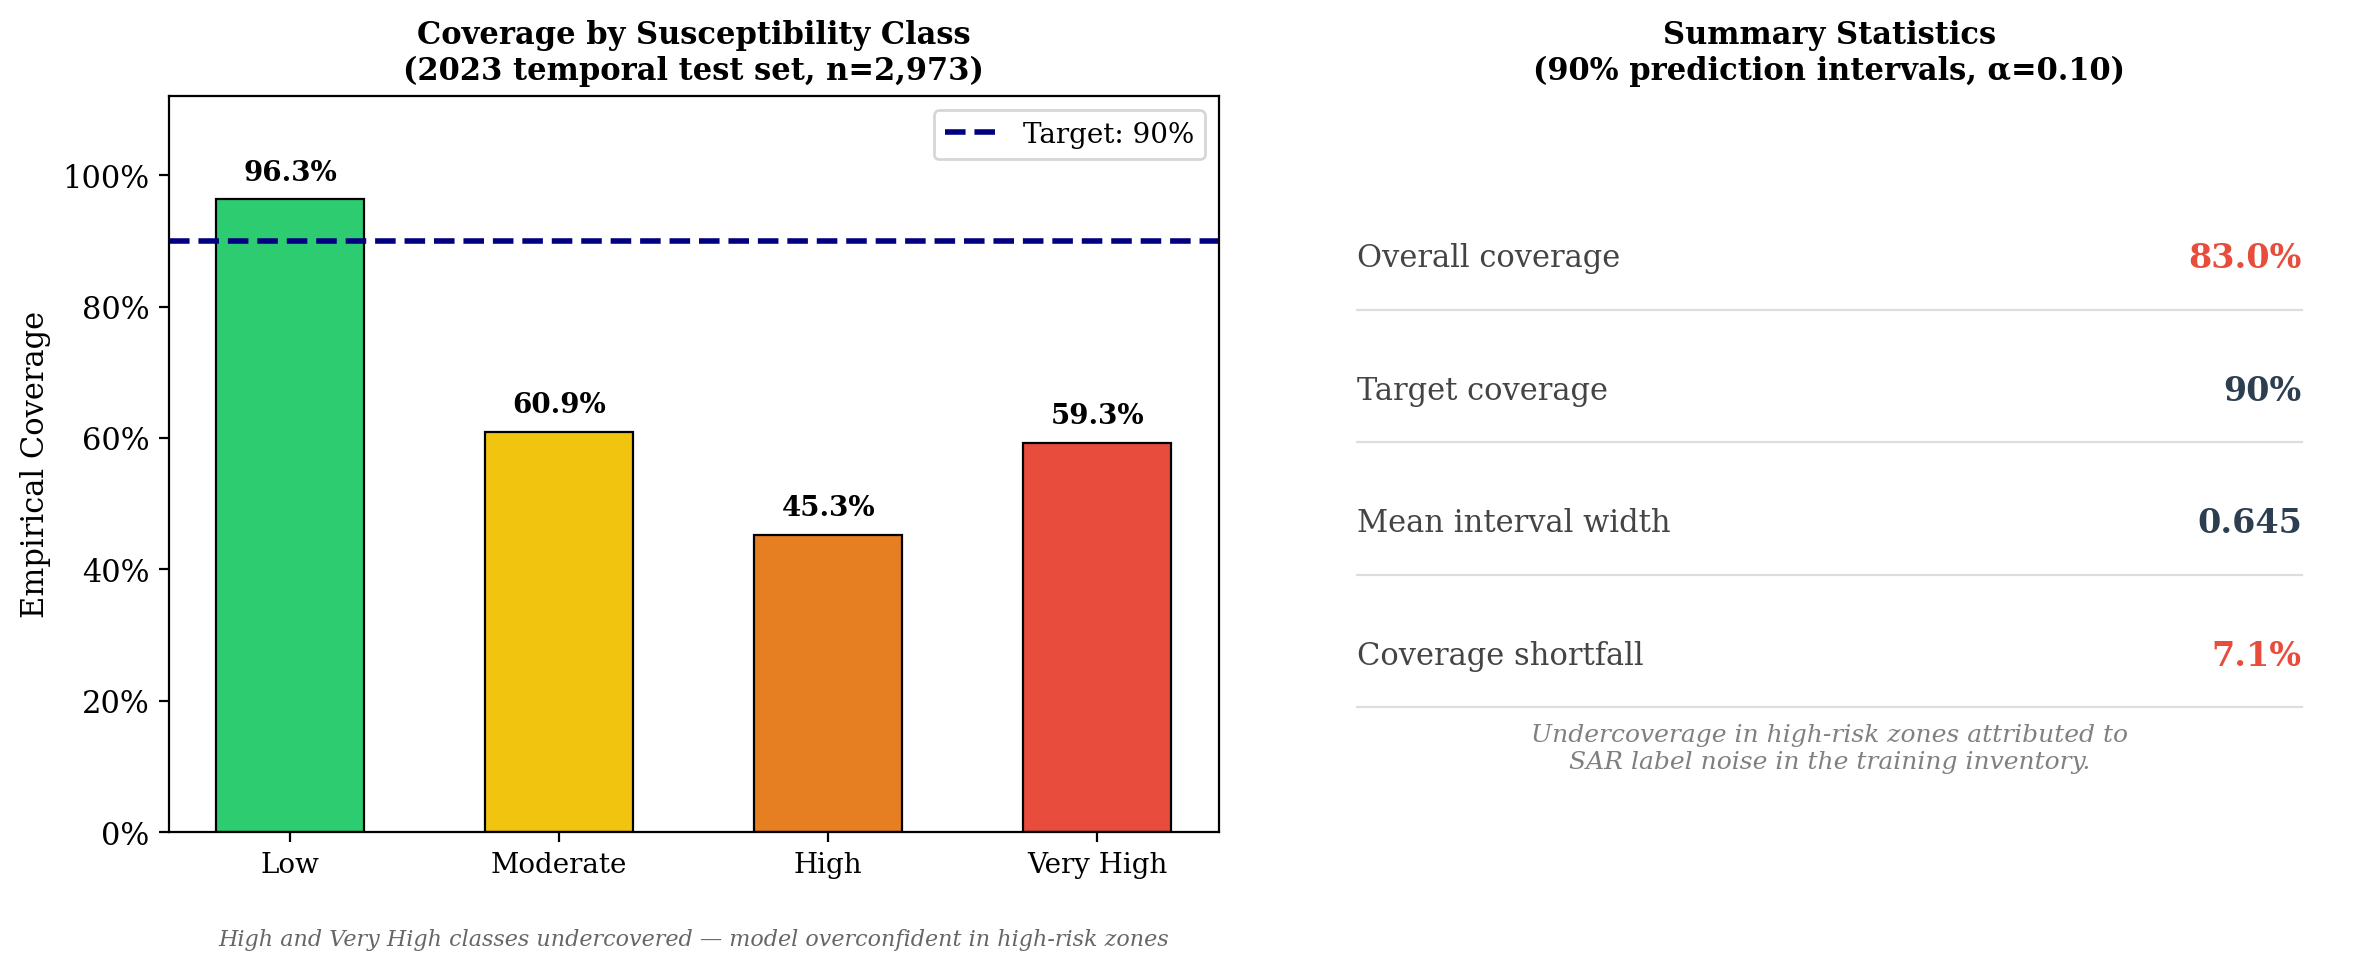
\includegraphics[width=0.85\textwidth]{../results/paper_figures/fig10_conformal_coverage.png}
  \caption{%
    \textbf{Figure 10:} Conformal prediction coverage analysis.
    \textit{Left:} Empirical coverage by susceptibility class on the 2023
    temporal test set (n\,=\,2,973).
    Dashed line: target 90\% coverage.
    Low susceptibility achieves 96.3\% coverage; High and Very High classes
    are undercovered (45--59\%), attributable to SAR label noise in the high-risk regime.
    \textit{Right:} Overall coverage (82.9\%), mean interval width (0.32),
    and validity summary.
  }
  \label{fig:conformal_coverage}
\end{figure}
